\documentclass[12pt]{article}
\usepackage[hmargin={1in},vmargin={1in,1in},foot={.6in}]{geometry}   
\geometry{letterpaper}              
\usepackage{color,graphicx}
\usepackage{setspace}
\usepackage{amsmath}
\usepackage{amssymb}
\usepackage{varioref}
\usepackage{textcomp}
\usepackage{textcomp}
\usepackage{mflogo}
\usepackage{wasysym}
\usepackage[normalem]{ulem}
\usepackage{hyperref}
\usepackage{booktabs}
\usepackage{natbib}

\newcommand{\HRule}{\rule{\linewidth}{0.25mm}}

\usepackage{fancyhdr} % This should be set AFTER setting up the page geometry
\pagestyle{plain} % options: empty , plain , fancy
\lhead{Subjectivity predicts adjective ordering preferences}\chead{}\rhead{}
\renewcommand{\headrulewidth}{.5pt}
\lfoot{}\cfoot{\thepage}\rfoot{}
\newcommand{\txtp}{\textipa}
\renewcommand{\rm}{\textrm}
\newcommand{\sem}[1]{\mbox{$[\![$#1$]\!]$}}
\newcommand{\lam}{$\lambda$}
\newcommand{\lan}{$\langle$}
\newcommand{\ran}{$\rangle$}
\newcommand{\type}[1]{\ensuremath{\left \langle #1 \right \rangle }}

\newcommand{\bex}{\begin{exe}}
	\newcommand{\eex}{\end{exe}}
\newcommand{\bit}{\begin{itemize}}
	\newcommand{\eit}{\end{itemize}}
\newcommand{\ben}{\begin{enumerate}}
	\newcommand{\een}{\end{enumerate}}

\newcommand{\gcs}[1]{\textcolor{blue}{[gcs: #1]}}
\definecolor{Green}{RGB}{10,200,100}
\newcommand{\ndg}[1]{\textcolor{Green}{[ndg: #1]}}
\newcommand{\jd}[1]{\textcolor{red}{[jd: #1]}}

\title{Supplementary information for\\[25pt]
{\Large \textbf{Subjectivity predicts adjective ordering preferences}}}

\author{Gregory Scontras$^1$, Judith Degen$^2$, and Noah D.~Goodman$^2$\\[5pt]
{\small $^1$University of California, Irvine}\\ {\small $^2$Stanford University}}
\date{}

\begin{document}

\maketitle

\vspace{5pt}

\appendix

\section{Comparing subjectivity with alternative accounts of adjective order}

In the main text, we have described the success of adjective subjectivity in predicting ordering preferences for multi-adjective strings. In this supplement, we attempt to compare the predictions of adjective subjectivity with those of alternative proposals. Direct quantitative comparisons prove difficult because the investigations to date have been largely qualitative. 
%(Exceptions are \citet{martin1969}, who reports behavioral measures of ordering preferences, and \citet{wulff2003}, who reports corpus measures.)
%; these data are sufficient for suggesting a potential phenomenon, but we believe insufficient for fully understanding it. 
%The only large-scale empirical studies of ordering preferences are \citet{martin1969}, who reports behavioral measures, and \citet{wulff2003}, who reports corpus measures (i.e., relative frequencies). Our study marries these two approaches, using both behavioral measures and corpus analyses to arrive at clear estimates of the preferences themselves---showing that there are reliable \emph{quantitative} phenomena to be explained.
%There is even less empirical work on the factors that contribute to these ordering preferences. 
While many authors have made useful theoretical contributions,
most have not attempted to operationalize their hypotheses, let alone test them in large-scale behavioral studies.
Indeed, most authors report only their own intuitions or the intuitions of a handful of informants, using a small set of adjectives and nouns.\footnote{\citet{martin1969} is the exception, reporting behavioral measures of ordering preferences and four different aspects of adjective meaning that he hypothesized would predict these ordering preferences. The best-performing measure was adjective ``definiteness;'' it accounts for between 32\% and 55\% of the variance in his preference data. (He tested two different sets of twenty adjectives. Adjective definiteness accounted for 55\% of the variation in the ordering preferences for first set of adjectives; for second set, definiteness accounted for 32\% of the variation.) We have seen that subjectivity seems to fare better, and in addition our study uses more adjectives, more nouns, and two different operationalizations of subjectivity.} 

%Still, understanding the \emph{relative} success of subjectivity in predicting adjective order would aid in understanding its \emph{absolute} success. To that end, 

In order to facilitate comparison with the predictions of subjectivity, we attempt here to operationalize several previous accounts. We begin at the beginning, with the ``inherentness'' hypothesis from \citet{sweet1898} and \citet{whorf1945}, which we operationalize by using the design of an experiment from \citet{martin1969}. Then we look at subsectivity, a binary theoretical construct that some linguists have argued underlies ordering preferences \citep[e.g.,][]{truswell2009}. Finally, we try to find noun-specific ordering preferences that would support an account based on concept formation, and even attempt to operationalize a concept-formability metric \citep{McNally2004,bouchard2005,svenonius2008}. To preview the findings, we continue to find that subjectivity predicts ordering preferences with remarkable accuracy, while alternative approaches do significantly less well.

\subsection{The predictive power of inherentness}

Early accounts of adjective ordering proposed that the primary factor derterming order was the ``inherentness'' of the adjectives. We find perhaps the most eloquent formulation of this claim in the following quote from \cite[p.~5]{whorf1945}: 

\begin{quotation}
English adjectives form two main cryptotypes with sub-classes. A group referring to `inherent' qualities---including color, material, physical state (solid, liquid, porous, hard, etc.), provenience, breed, nationality, function, use---has the reactance of being placed nearer the noun than the other group, which we may call one of non-inherent qualities, though it is rather the residuum outside the first group---including adjectives of size, shape, position, evaluation (ethical, esthetic, or economic). These come before the inherent group, e.g. \emph{large red house} (not \emph{red large house}), \emph{steep rocky hill}, \emph{nice smooth floor}.
\end{quotation}

Unfortunately, most authors are content with merely asserting the claim concerning inherentness, not rigorously testing it. The single outlier is \cite{martin1969}; he documented that inherentness accounted for between 3\% and 14\% of the variation in the ordering preferences that he measured for 40 adjectives.  Still, to allow for a direct comparison of the predictions of subjectivity with those of inherentness, it was necessary to measure their values for the same set of materials. Therefore, we ran a version of \citeauthor{martin1969}'s original task using the adjectives and nouns from Expt.~1, and included a replication of our subjectivity experiment.% to allow for a direct comparison of the predictions of subjectivity with those of inherentness.%\jd{So what was Martin?s result? Why are we doing the same thing if he already did it? (Or is this already discussed in the main paper?)}

\paragraph{Participants.} We recruited 72 participants through Amazon.com's Mechanical Turk. Participants were compensated for their participation.

\paragraph{Design and methods.} Participants were randomly assigned to one of two conditions: \emph{inherentness} (n=41) or \emph{subjectivity} (n=31). For the inherentness condition, participants rated the ``essentiality'' of adjective-noun object descriptions; they were told that they would be ``asked to decide how essential the adjective is to the meaning of the noun which it modifies, that is, how substantive or inherent the adjective seems in its meaning.'' This language comes from \citeauthor{martin1969}'s original ``substantiveness'' task instructions \citep[Expt.~VII]{martin1969}. Participants indicated their rating using a slider with endpoints labeled ``completely nonessential'' (coded as 0) and ``completely essential'' (coded as 1).

The subjectivity condition was a replication of our original ``subjectivity'' experiment, modified to match the inherentness task. Participants rated the ``subjectivity'' of adjective-noun object descriptions (and not adjectives in isolation; cf.~our \emph{Expt.~1: Subjectivity}); they were told that they would be ``asked to decide how subjective the adjective seems in its meaning.'' Participants indicated their rating using a slider with endpoints labeled ``completely objective'' (coded as 0) and ``completely subjective'' (coded as 1).

Participants completed a total of 26 trials, one for each of the adjectives in Table 1; nouns were chosen at random from the list in Table 1. All 72 participants indicated that they were native speakers of English; we analyze their data below.

\paragraph{Results.} We averaged the inherentness and subjectivity scores for each adjective. Fig.~\ref{fig:inherentness} plots mean inherentness (\emph{left}) and subjectivity (\emph{right}) scores against the inferred distance naturalness scores from \textit{Expt.~1: Ordering preferences}. As Fig.~\ref{fig:inherentness} demonstrates, inherentness does little to predict ordering preferences, accounting for 0.0\% of the variance in the naturalness ratings ($r^2${=}0.00, 95\% CI [0.00,  0.02]). However, we have replicated the success of adjective subjectivity, which accounts for 75\% of the variation in the naturalness ratings ($r^2${=}0.75, 95\% CI [0.53,  0.84]).

\renewcommand\thefigure{A.\arabic{figure}}
\begin{figure}
	\centering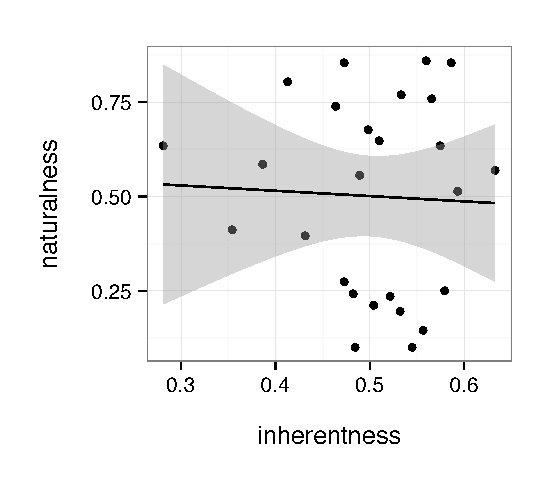
\includegraphics[width=3in]{plots/expt1-inherentness-naturalness.eps}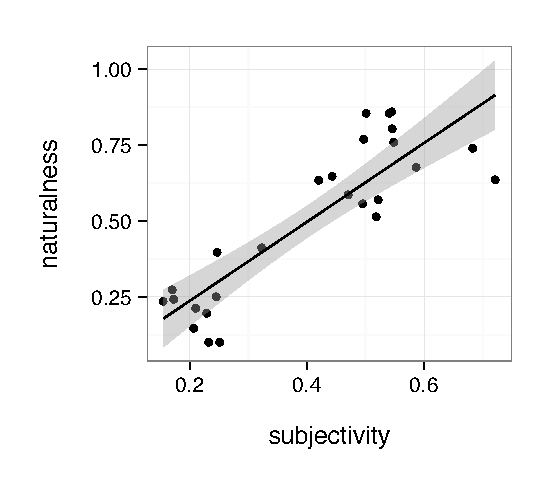
\includegraphics[width=3in]{plots/expt1-subjectivity2-naturalness.eps}
	\caption{Mean naturalness ratings plotted against mean inherentness (\emph{left}) and subjectivity (\emph{right}) scores for each of the 26 adjectives tested. Here and in all other graphs, gray ribbons represent 95\% confidence intervals using a t-based approximation.}\label{fig:inherentness}
\end{figure}

\paragraph{Discussion.} Using a modified version of \citeauthor{martin1969}'s (\citeyear{martin1969}) task measuring adjective inherentness, we failed to find \emph{any} correlation between inherentness and ordering preferences for our set of 26 adjectives. Indeed, our findings match \citeauthor{martin1969}'s own, namely that inherentness is a poor predictor of adjective ordering preferences. %\jd{Maybe because his task is shitty\dots} 
We also measured adjective subjectivity, which allows for a direct comparison of the two predictors: whereas inherentness accounted for no variation, subjectivity accounted for 75\% of the variation in our ordering preferences. Despite the many claims to its success in the literature \citep[e.g.,][]{sweet1898,whorf1945,kemmerer2000}, adjective inherentness does little (or nothing) to explain the observed regularities in adjective order. However, subjectivity continues to predict ordering preferences.



\subsection{Subjectivity vs.~subsectivity}

Next, we turn to a more abstract but no less popular factor meant to account for ordering preferences: the logical distinction between intersectivity and subsectivity. Semanticists argue that adjectives split on the basis of how they modify the nouns with which they compose \citep[for discussion, see][]{kamppartee1995}. Some adjectives are \emph{intersective}: the outcome of their modification is the intersection of the nominal denotation with the adjectival denotation, as in the following example, where \emph{carnivorous mammal} describes those things that hold the property of being carnivorous and of being a mammal.

\begin{align*} 
\sem{carnivorous} &= \{x : carnivorous(x)\}\\
\sem{mammal} &= \{x : mammal(x)\}\\
\sem{carnivorous mammal} &= \{x : carnivorous(x)\ \&\ mammal(x)\}\\
& =\sem{carnivorous} \cap \sem{mammal}
\end{align*}

\noindent Other adjectives are \emph{subsective}: rather than intersecting with a nominal denotation, the outcome of subsective modification is a subset of the nominal denotation, which is used to determine the comparison class for the adjective. Subsective adjectives depend on the nominal with which they compose to fix their meaning. Take \emph{skillful}: a skillful surgeon is not necessarily a skillful violinist, but a skillful surgeon is necessarily a surgeon:

\begin{align*} 
\sem{skillful surgeon} & \subseteq \sem{surgeon}
\end{align*}

\noindent Finally, there are those adjectives that are neither clearly intersective nor clearly subsective. The most obvious cases are so-called \emph{privative} adjectives like \emph{fake}, which require that the outcome of modification is a proper complement of the nominal denotation: a fake gun is not a gun.  More generally, these non-intersective, non-subsective adjectives preclude the inference that the things described hold the property named by the noun:

\begin{align*} 
\sem{fake gun} & \nsubseteq \sem{gun}\\
\sem{former senator} & \nsubseteq \sem{senator}
\end{align*}

What matters for present purposes is that some authors assume that the means of modification determines adjective order, such that intersective adjectives occur closer to the noun than subsective adjectives. We find the clearest statement of this claim in \cite{truswell2009}, who assumes that hierarchical dominance leads to linear precedence:

\begin{quotation}
\noindent\ben
	\item Subsective adjectives dominate intersective adjectives. \item Modal [(i.e., non-subsective)] adjectives are freely ordered with respect to subsective and intersective adjectives, although they tend to dominate both classes.
	\een
\end{quotation}

\noindent According to \citeauthor{truswell2009}, intersective adjectives occur closest to the modified noun, subsective adjectives occur farther than intersective adjectives, and non-subsective adjectives are freely ordered, despite their tendency to occur farthest of all.\footnote{See \citet{Sproat1991} for a similar claim, which uses the language of the ``relative'' (i.e., subsective) vs.~``absolute'' (i.e., intersective) distinction (cf.~\citealp{siegel1976}).} 

Subsectivity is not a true competitor to the subjectivity hypothesis, in two ways. 
Most importantly, the intersective--subsective distinction is a binary one, but there is systematic \emph{graded} behavior in the ordering of adjectives. The binary distinction could at best explain the first bit of ordering preference data (though this could be a useful start).
Second, the intersective--subsective distinction is a theoretical construct, not a natural human concept; it takes consultation with a trained linguist to fix the status of a given adjective.\footnote{To see what it would take to operationalize the distinction as a behavioral measure, see our attempt at operationalizing concept formability in Section \ref{operationalize} below.} This makes it theoretically useful, but behaviorally problematic.
%Compare this with subjectivity, where we have seen the success of two behavioral measures with naive participants. 
Still, we attempted to compare the predictions of the two proposals. To do so, we coded our adjectives as either \emph{subsective}, \emph{intersective}, or \emph{other} using \citeauthor{truswell2009}'s classifications: shape, color, nationality, and material adjectives were coded as \emph{intersective}; all other adjectives were coded as \emph{subsective}, except for the non-intersective class ``X'' adjectives from Expt.~2, which we coded as \emph{other}.

The first thing to note is that the two predictors (i.e., subjectivity and subsectivity) are extremely highly correlated (Expt.~1: $r^2${=}0.89, 95\% CI [0.74,  0.94]; Expt.~2: $r^2${=}0.52, 95\% CI [0.35,  0.65]). This correlation should come as no surprise, given that the intersective--subsective distinction hangs on the context sensitivity of the adjective: intersective adjectives have fixed interpretations (i.e., they are maximally objective), while the interpretation of subsective adjectives varies with the modified noun. Given this high correlation and the observed success of subjectivity in predicting ordering preferences, we expect subsectivity to do well in predicting ordering preferences. However, the binary nature of the subsectivity predictor cannot account for the variation \emph{within} the classes of subsective and intersective adjectives. 

\renewcommand\thefigure{A.\arabic{figure}}
\begin{figure}
	\centering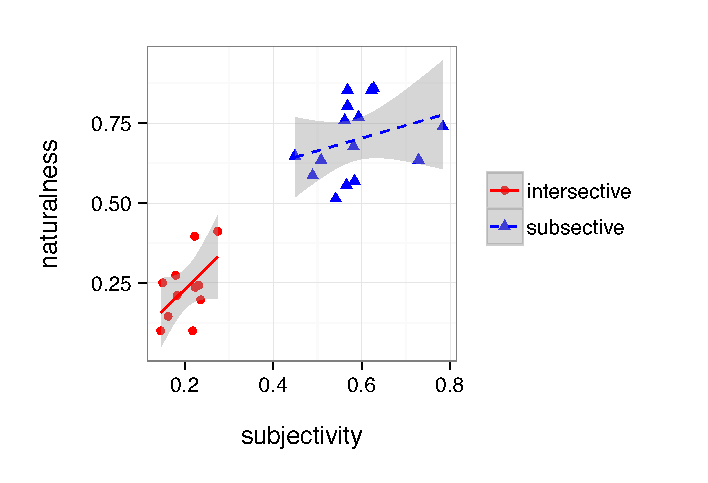
\includegraphics[width=4.5in]{plots/expt1-subjectivity-subsectivity.eps}\\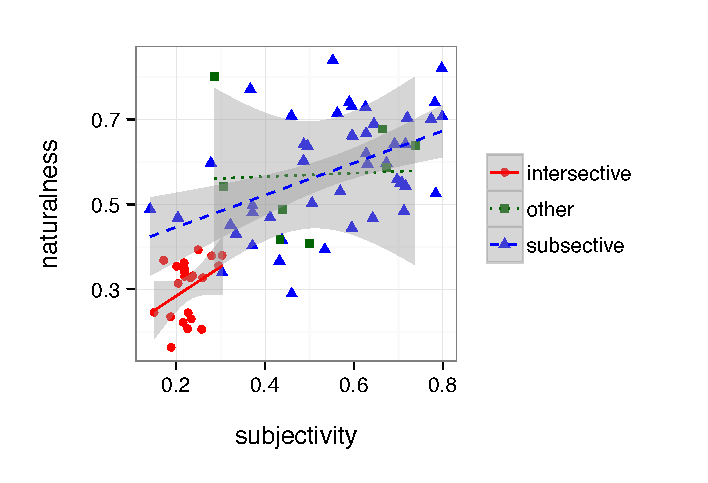
\includegraphics[width=4.5in]{plots/expt3-subjectivity-subsectivity.eps}
	\caption{Mean naturalness ratings plotted against mean subjectivity scores grouped by subsectivity for the original set of 26 adjectives tested in Expt.~1 (\emph{top}) and the expanded set of 78 adjectives tested in Expt.~2 (\emph{bottom}).}\label{fig:subsectivity}
\end{figure}

Fig.~\ref{fig:subsectivity} plots adjective subjectivity scores against naturalness ratings from Expt.~1 (\emph{top}) and Expt.~2 (\emph{bottom}), grouping adjectives by subsectivity class. To evaluate the role of subjectivity \emph{over and above subsectivity} in predicting ordering preferences, we performed a nested linear model comparison. The models  %\jd{What sorts of models? Linear regression with predictors for subsectivity / subsectivity and subjectivity (just main effects or interactions as well?)} 
we compared predicted naturalness ratings by \textsc{subsectivity} only, or by \textsc{subsectivity} and \textsc{subjectivity}. The model comparison revealed that subjectivity does explain additional variance in ordering preferences beyond the intersective--subsective distinction (Expt.~1: $F(1,2337)=25.28, p<0.001$; Expt.~2: $F(1,23786)=361.78, p<0.001$): as Fig.~\ref{fig:subsectivity} shows, even within the subsectivity classes, subjectivity continues to predict ordering preferences. Thus, we continue to find support for the subjectivity hypothesis.  Performing the comparison in the reverse, we see that subsectivity also explains variance over and above subjectivity (Expt.~1: $F(1,2337)=36.89, p<0.001$; Expt.~2: $F(2,23786)=242.60, p<0.001$). That is, both subjectivity and subsectivity explain independent variance in ordering preferences---a finding which warrants future study.


\subsection{Testing compositional accounts}

Compositional accounts of ordering preferences hold that the fundamental factor in predicting adjective ordering is whether or not an adjective is used to form a complex concept/subkind description: first you form the concept, then you modify it with additional adjectives \citep{McNally2004,svenonius2008}.\footnote{\cite{bouchard2005} makes a similar claim, namely that the formation of complex concepts can override adjective ordering preferences.} 
This would imply that an interaction between the noun and a modifying adjective---whether they combine to form a complex concept---should have a large influence on adjective ordering. 
Indeed, a more general hypothesis is that \emph{some} interaction between a noun and adjective will influence how closely the adjective is placed to that noun. This interaction could be caused by concept-formation, differential subjectivity, or other factors. We tested for such an interaction in the results of Expts.~1 and 2; we present each analysis in turn.

\textbf{Expt.~1:} To evaluate the role of specific noun information in determining ordering preferences, we performed a nested linear model comparison of our ordering preference data. The models predicted naturalness ratings either by \textsc{adjective} (i.e., the adjective farthest from the noun) only, or by \textsc{adjective} together with its interaction with \textsc{noun} (i.e., the modified noun).
The model comparison revealed that noun-specific ratings did not explain any additional variance in ordering preference above and beyond adjective-level ratings ($F(234,2080) = 1.10, p < 0.15$).  Thus, we fail to find evidence of noun-specific effects on ordering preferences in our materials.

\textbf{Expt.~2:} We performed the same nested model comparison on the results of our second ordering preference experiment. Once again, the model comparison revealed that noun-specific ratings did not explain any additional variance in ordering preference 
%above and 
beyond adjective-level ratings ($F(9676,11593) = 1.02, p < 0.14$). However, participants were not ignoring the nouns altogether. To see whether nouns had an effect on sense rates, we performed another nested linear model comparison. This time, the models we compared predicted the sense of an object description (i.e., whether participants indicated that the description ``made sense'') either with the two \textsc{adjectives} only, or with the \textsc{adjectives} and the \textsc{noun}. The model comparison revealed that noun information does explain additional variance in sense rates beyond the two adjectives involved ($F(165,11267)=2.03, p<0.001$), suggesting that participants were paying attention to the nouns in the object descriptions they encountered.\\

\noindent Having found that noun-specific naturalness did not explain any variance in ordering preference above and beyond adjective-level naturalness, we lack evidence suggesting that ordering preferences depend on the modified noun at all. %Looking in more detail, there were two adjective-noun pairs in our data with trends in the predicted direction: the naturalness ratings for \emph{hard} and \emph{soft} suggested a preference to occur closer to the noun \emph{cheese}. (Plausibly because hard and soft cheeses are natural kinds.) While these adjective-noun interactions do not survive correction for multiple comparisons in our statistical analysis, they do indicate that a different set of materials might reveal by-noun effects on ordering preference. 
In what follows, we follow up on this result, first with a new set of materials that were chosen to maximize the probability of noun effects on ordering preferences, and then with our attempt at operationalizing a concept-formability metric.

\subsubsection{In search of noun effects}

This experiment was a direct replication of \emph{Expt.~1.1 Ordering preferences}, using a different set of nouns. We aimed to choose nouns that formed idiomatic, complex concepts with our set of 26 adjectives (along the lines of \emph{bad apple} or \emph{blue cheese}).  %\jd{Give an example?} 
Complex concepts tend to be described using the two-word name, yielding more occurrences of this bigram than would be expected from the unigram frequencies of the noun and adjective. This provided a way to extract candidate complex concepts from corpora.

 %with the given adjectives and therefore yield effects on ordering preferences.

\paragraph{Participants.}

We recruited 50 participants through Amazon.com's Mechanical Turk crowd-sourcing service. Participants were compensated for their participation.

\paragraph{Design and methods.}

The design was identical to our original naturalness ratings experiments: participants were asked to indicate which of two object descriptions sounded more natural, using a sliding scale. Each description featured a noun modified by two adjectives; description pairs contained the same words with the relative adjective order reversed (e.g., ``the big blue thing'' vs.~``the blue big thing''). Adjectives were chosen at random from the set in Table 1. The nouns were a smaller set of five (compared to the original ten). Nouns were chosen to maximize the probability of detecting noun-specific effects on adjective ordering preferences. In particular, we expected that nouns that are likely to form complex concepts should be 
highly collocational with that adjective. We thus searched for nouns that occur in particular adjective-noun phrases more frequently than predicted by the individual noun and adjective probabilities; in other words, nouns whose adjective-noun combinations were under-predicted by their individual word probabilities. 

To find these nouns, we estimated the probability $p(A)$ of each adjective from our set of 26 by computing its relative frequency in an adjective-noun sequence in the BNC. We then computed the relative frequency of each noun $p(N)$ occurring in an adjective-noun sequence. Finally, we estimated the predicted joint probability of each adjective-noun combination by taking the product of each individual probability estimate: $\hat{p}(A,N) = p(A)\cdot p(N)$. Comparing  $\hat{p}(A,N)$ to the empirically estimated $p(A,N)$ establishes which adjective-noun combinations are under-predicted---more collocational---and thus likely to name complex concepts. We then restricted nouns to those 50 that maximize the observed range of under-predictedness while simultaneously requiring that each noun be attested to occur with at least 11 of the 26 adjectives; from these 50 nouns, we selected the following four: \emph{apple, cheese, eyes, hair}.\footnote{We restricted to a small subset of the 50 target nouns in order to maximize statistical power to identify noun effects on ordering.} (Recall that \emph{cheese} occurred in our original materials, where it suggested possible by-noun effects with the adjectives \emph{hard} and \emph{soft}.) To these four nouns we added a fifth: \emph{thing}.
While \emph{thing} did not occur in the top 50, it did occur naturalistically with the most adjectives (23) out of the set of 26, thus allowing it to serve as a filler for the various object descriptions. The selected nouns, together with the number of adjectives they occur with, their range of ratios of empirical to predicted joint probabilities, and their minimum / maximum ratios, are shown in Table \ref{tab:nouns}.

\renewcommand\thetable{A.\arabic{table}}
\begin{table}
\centering
\begin{tabular}{l c c c c}
\toprule
Noun & \# of adjectives & range of ratios & minimum ratio & maximum ratio\\
\midrule
thing & 23 & 10.4 & 0.1 & 10.5 \\
eyes & 18 & 120.6 & 0.12 & 120.7 \\
hair & 15 & 82.9 & 0.03 & 83.0 \\
cheese & 13 & 114.0 & 0.4 & 114.4 \\
apple & 11 & 674.0 & 1.1 & 675.1 \\
\bottomrule
\end{tabular}
\caption{For each chosen noun, the number of adjectives (out of 26) that it occurs with; and for each adjective $A$ that the noun occurs with, the range of ratios $p(A,N) / \hat{p}(A,N)$ (empirical to predicted probability of occurrence); the minimum ratio; and the maximum ratio.}
\label{tab:nouns}
\end{table}




\paragraph{Results.}

To evaluate the role of specific noun information in determining ordering preferences, we performed the same nested linear model comparison from our original naturalness ratings experiment (\emph{Expt.~1: Ordering preferences}). The models we compared predicted naturalness ratings either by \textsc{adjective} (i.e., the adjective farthest from the noun) only, or by \textsc{adjective} together with its interaction with \textsc{noun} (i.e., the modified noun).
The model comparison revealed that noun-specific ratings did not explain any additional variance in ordering preference beyond adjective-level ratings ($F(104,2366) = 1.07, p < 0.30$).  Thus, we again fail to find evidence of noun-specific effects on ordering preferences in our new materials. 


%\subsection{Subjectivity}
%
%We next set out to replicate the finding that subjectivity predicts adjective ordering preferences in our new materials.
%
%\paragraph{Participants.}
%
%We recruited 40 participants through Amazon.com's Mechanical Turk crowd-sourcing service. Participants were compensated for their participation.
%
%\paragraph{Design and methods.}
%
%This experiment was a direct replication of our original faultless disagreement subjectivity experiment (Experiment 3), using the new set of nouns from the previous experiment.

%\paragraph{Predicting adjective order.}

Given the lack of noun effects on ordering preferences, we should continue to find that adjective subjectivity predicts ordering preferences. Indeed, it does: adjective subjectivity scores (obtained in \emph{Expt 1.2 Subjectivity}) account for  85\% of the variance in the new naturalness ratings ($r^2${=}0.85, 95\% CI [0.64,  0.93]; Fig.~\ref{fig:subjectivity}). 
%Faultless disagreement scores account for  84\% of the variance in the new naturalness ratings ($r^2$ 0.84, 95\% CI [0.64,  0.91]; Fig.~\ref{fig:faultless}). 
As with our original materials, more subjective adjectives are preferred farther from the noun.


\renewcommand\thefigure{A.\arabic{figure}}
\begin{figure}
	\centering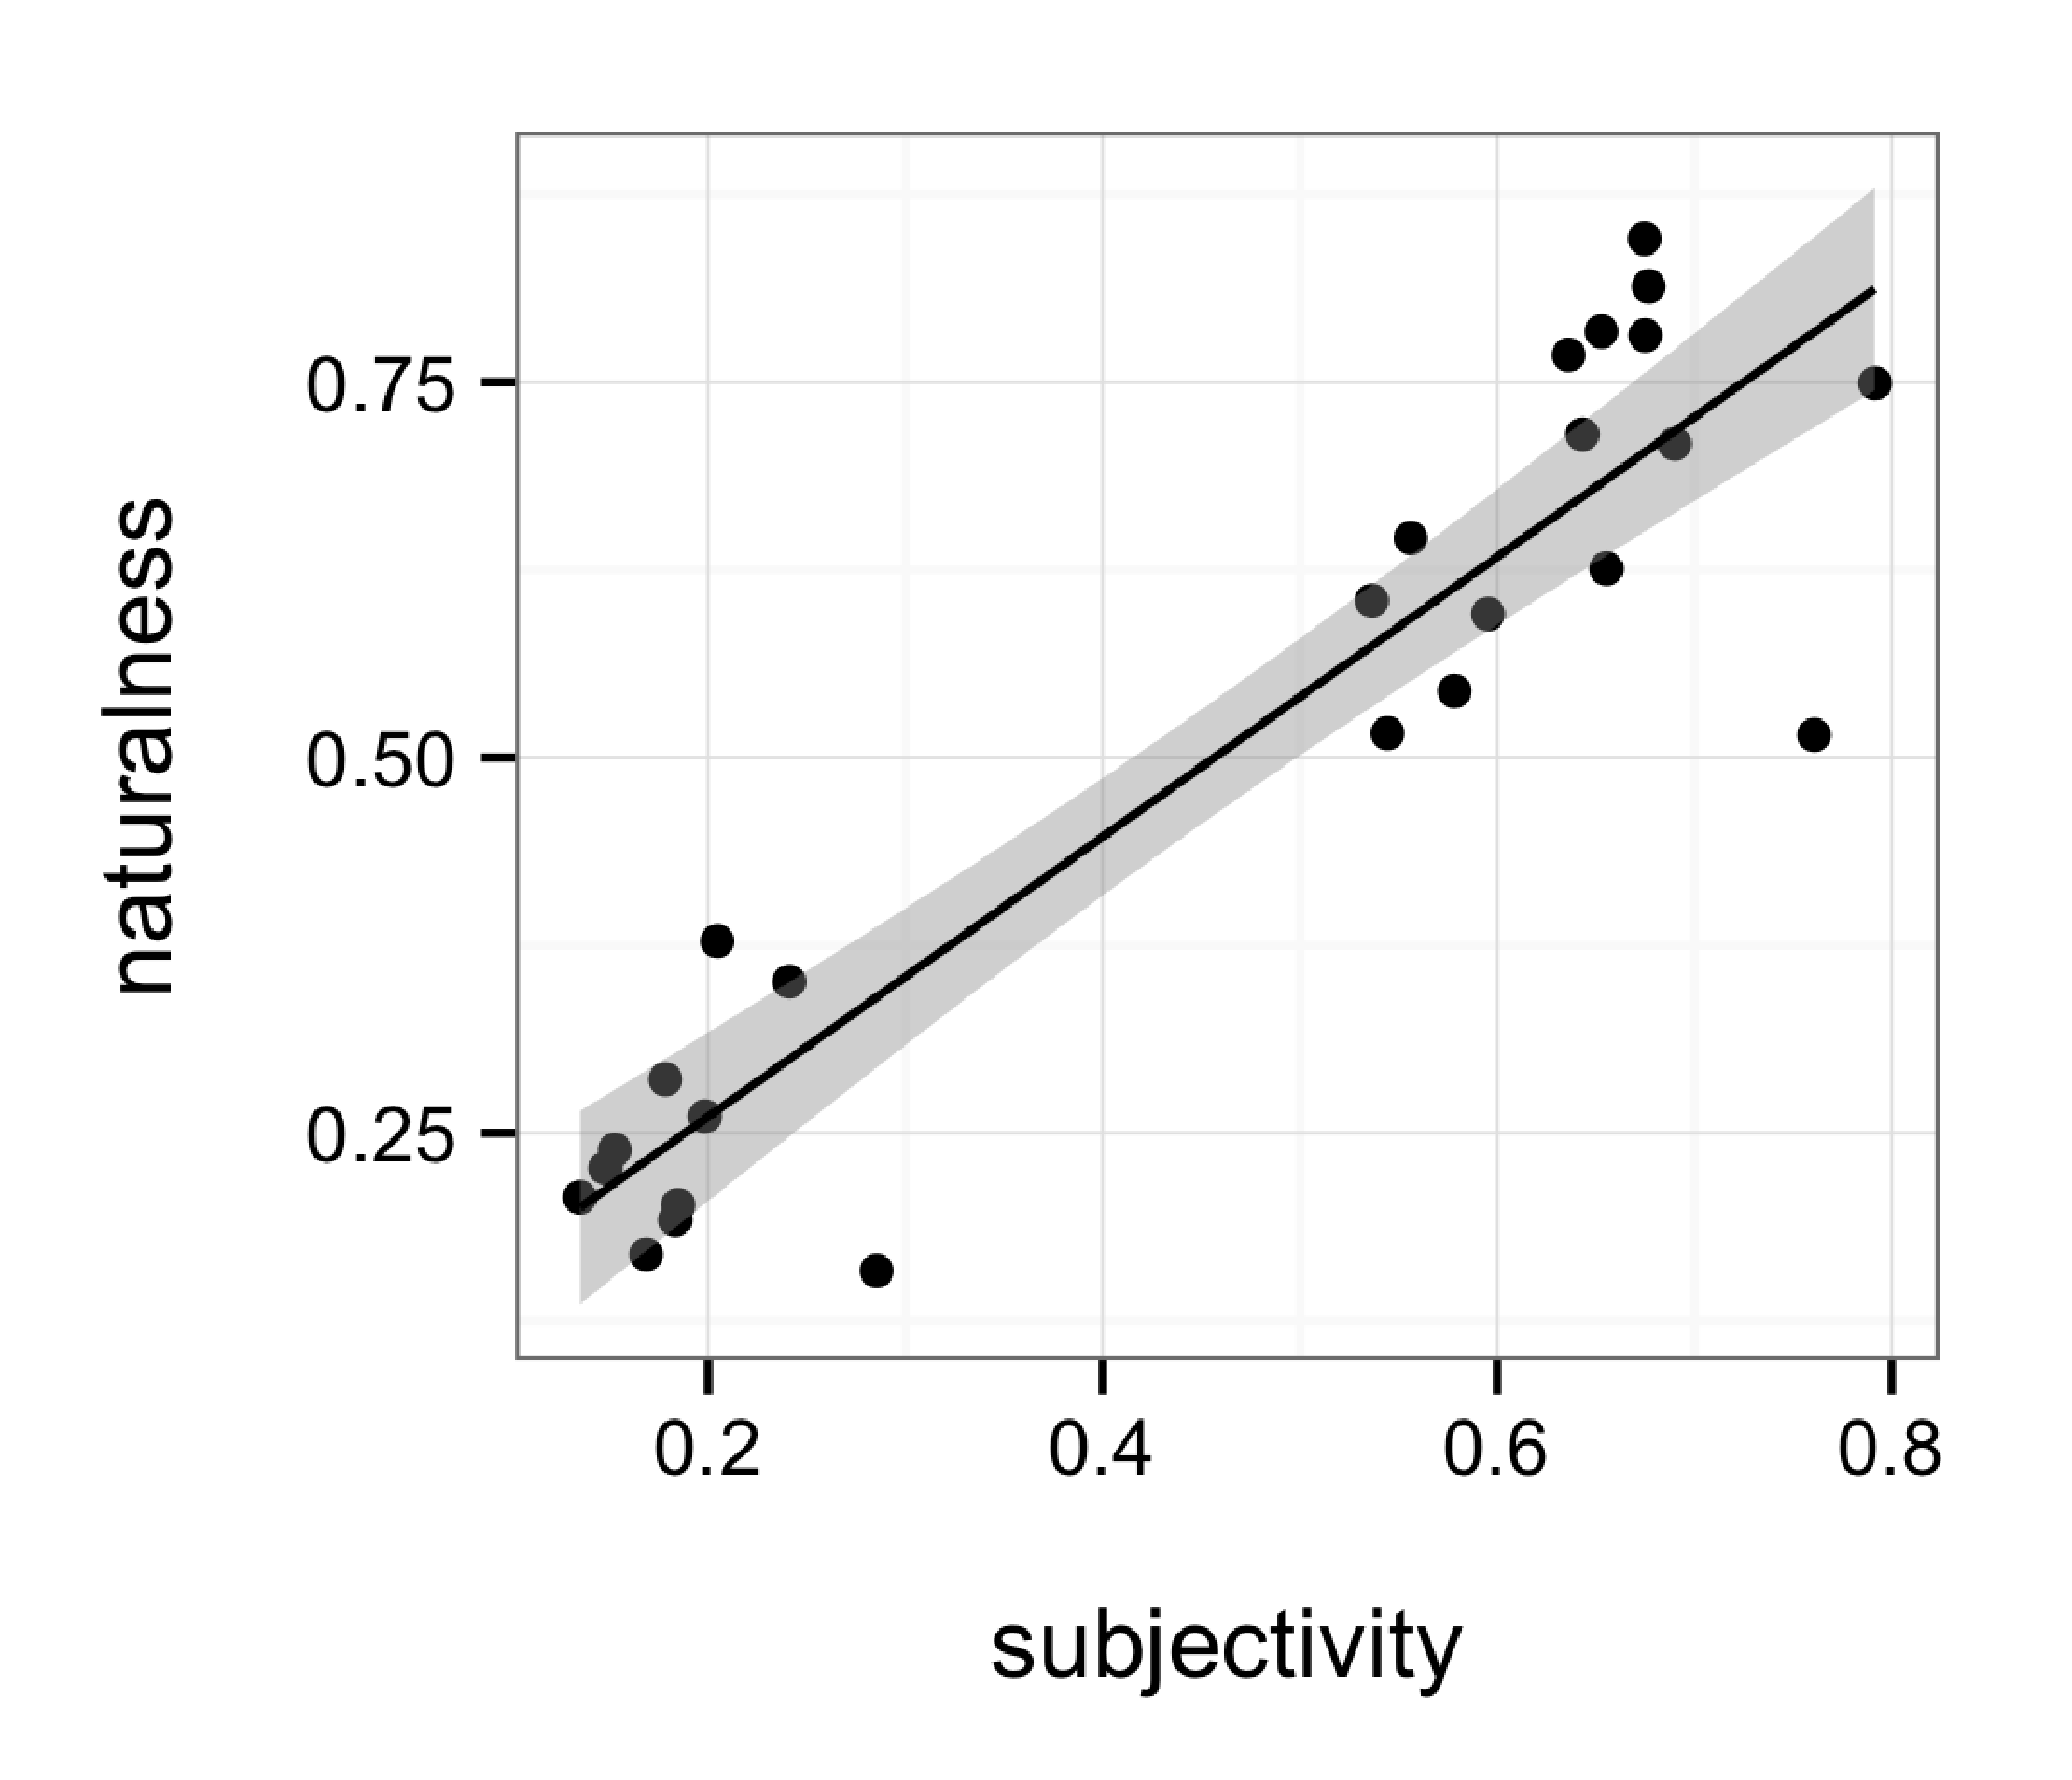
\includegraphics[width=3.5in]{plots/naturalness-subjectivity-new-nouns.eps}
	\caption{Mean naturalness ratings plotted against mean subjectivity scores for each of the 26 adjectives tested in the new order preference experiment.}\label{fig:subjectivity}
\end{figure}

\paragraph{Discussion.} Using nouns chosen to maximize the probability of complex concepts formed with our 26 adjectives, we failed to find evidence that adjective ordering preferences depend on the modified noun. We do continue to find that subjectivity predicts ordering preferences. Thus, we failed to find evidence in support of compositional accounts of ordering preferences, which hold that the most important factor in determining order is whether or not an adjective forms a complex concept with the noun it modifies. 
It remains possible that noun-effects (and hence effects of concept composition)  %\jd{Couldn?t there be noun effects that aren?t effects of concept composition?} 
would be found with a different set of adjectives. Moreover, there could be noun effects that are not related to concept composition. 
However, this already suggests that the effect of modified nouns explains only a small part of the overall story of adjective order, while subjectivity is a robust predictor.



\subsubsection{Operationalizing concept-formability} \label{operationalize}

Failing to find support for the most general prediction of the compositional account, namely an effect of nouns on ordering preferences, we tried a more targeted approach: operationalizing a concept-formability metric, and testing its predictions on the adjective ordering preferences that we measured in \emph{Expt.~1: Ordering preferences}. As with the studies in our paper, the work lies in operationalizing the abstract notion of whether or not an adjective-noun combination tends to form a complex concept. The literature on the topic presupposes that intuitions about concept formability are systematic and generalizable \citep{McNally2004,svenonius2008}; the closest we found in these papers to a proposal for an empirical measure of this factor is the following distinction.

According to \citeauthor{McNally2004}, the key issue is one of entailment. When an adjective modifies a noun intersectively, the objects described hold both the property named by the noun and the property named by the adjective: a ``male architect'' is both male and an architect \citep[p.~179, ex.~2]{McNally2004}. When an adjective and a noun combine to form a complex concept (i.e., a subkind description), the objects described hold the property named by the noun, but not necessarily the property named by the adjective; the modification is (ostensibly) subsective. The authors give the Catalan example \emph{arquitecte t\`{e}cnic} ``technical architect,'' which names a kind of architect but not necessarily technical things (\citealp[p.~179, ex.~1]{McNally2004}; cf.~the discussion of \emph{wild rice} in \citealp{svenonius2008}).\footnote{This distinction should ring familiar from the discussion of intersective vs.~subsective modification above. Indeed, as \citeauthor{McNally2004} characterize it, concept formability is closely related to the intersective/subsective distinction, and the current experiment operationalizes both.} 
Using our original set of materials, we tested whether the objects named by an adjective-noun description hold 1) the property named by the adjective, and 2) the property named by the noun.

%Suppose the fundamental factor in predicting adjective ordering is whether an adjective is used to form a complex concept/subkind description or not.

%We find this hypothesis intriguing---perhaps concept-formability indeed determines ordering preferences (and therefore correlates with subjectivity)? The semantic analysis given by these authors to adjectives that form complex concepts requires them to compose first with nouns, before run-of-the-mill intersective adjectives; thus, the fundamental factor in predicting adjective ordering ought to be whether an adjective forms a complex concept. Does concept-formability predict ordering preferences?


\paragraph{Participants.} We recruited 40 participants through Amazon.com's Mechanical Turk.  Participants were compensated for their participation.

\paragraph{Design and methods.} Participants were presented with 26 adjective-noun object descriptions. They were instructed to ``consider the things that might be described'' as \texttt{adjective-noun} (e.g., ``round desks''), then rate how likely it is that the things described 1) hold the \texttt{adjective} property (e.g., ``Are those things round?''), and 2) hold the \texttt{noun} property (e.g., ``Are those things desks?''). %\jd{Why isn?t this just a test of inter-/subsectivity?}
 Participants indicated their probability ratings using sliders with endpoints labeled with ``definitely not'' (coded as 0) and ``definitely'' (coded as 1). 
 %\footnote{The full experiment is \href{http://web.stanford.edu/~scontras/adjective_ordering/experiments/9-concept-formability/concept-formability.html}{viewable online here}.} 
 All 40 participants indicated that their native language was English; we report their results below.

\paragraph{Results.} %We averaged probability scores for each adjective. 
To ensure that we did not wash out the noun-specific effects that this analysis was supposed to pick up, we computed two sets of adjective probability scores: 1) adjective-noun probability scores that simply averaged ratings across participants, and 2) adjective probability scores that collapsed over the modified noun. 
%\jd{Wait, by averaging, don?t you wash out the noun-specific effects which this analysis is supposed to pick up on?} 
Fig.~\ref{fig:concept} plots the adjective-noun (\emph{left}) and adjective (\emph{right}) scores against the naturalness ratings from \emph{Expt.~1: Ordering preferences}. According to the predictions of the compositional account, lower adjective (or adjective-noun) probability should lead to lower naturalness (i.e., a decreased preference to place the adjective farther from the noun): 
%\jd{repeat why (ie, higher naturalness of what?)}: 
as the property named by an adjective is less likely to apply straightforwardly to the objects named, the probability that the adjective forms a complex concept with the noun it modifies increases. %\jd{so\dots what is the connection between this and naturalness?}. 
While we do observe this trend for the simple adjective scores in Fig.~\ref{fig:concept} (\emph{right}), we also see that adjective probability scores predict just 8\% of the variance in our preference data (r$^{2}=0.08$; 95\% CI [0.00,  0.33]). The adjective-noun scores perform even worse, accounting for none of the variance in the adjective-noun preference data (r$^{2}=0.00$; 95\% CI [0.00,  0.00])


\renewcommand\thefigure{A.\arabic{figure}}
\begin{figure}
	\centering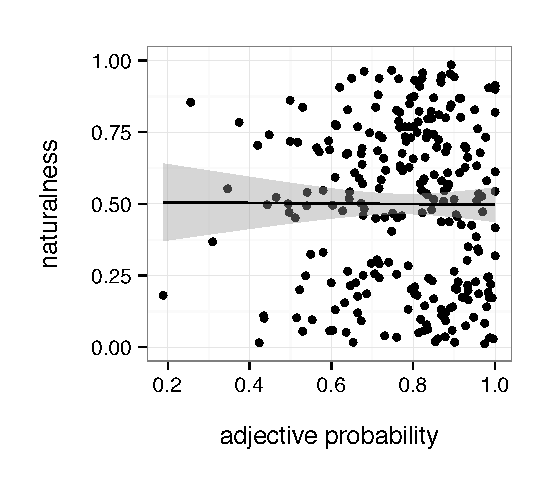
\includegraphics[width=3in]{plots/naturalness-concept-noun-pred.eps}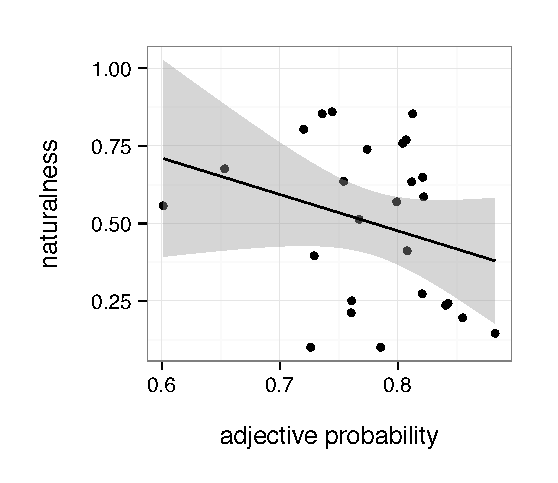
\includegraphics[width=3in]{plots/naturalness-concept-adjective.eps}
	\caption{Mean naturalness ratings plotted against mean adjective probability (i.e., concept-formability) scores for each of the 26 adjectives tested. In computing mean adjective probability, we either took into account (\emph{left}) or collapsed over (\emph{right}) specific noun information.}\label{fig:concept}
\end{figure}

\paragraph{Discussion.} Recall that at its worst, subjectivity predicts 70\% of the variance in our preference data. 
While it is quite possible that concept-formability plays an important role for some cases (such as \emph{arquitecte t\`{e}cnic}), we did not find evidence that it was critical to ordering preferences in our broad set of items. 

\subsection{Conclusion}

We have compared the subjectivity hypothesis with the predictions of three alternative accounts of adjective order: inherentness, subsectivity, and concept-formability. Our results demonstrate the robust replicability of the success of subjectivity in predicting adjective order. The results also demonstrate that the alternative accounts we considered add little to our understanding of ordering preferences: everywhere we looked, subjectivity continued to best predict ordering preferences. %while the alternatives did not add explanatory value, with the exception of inter/subsectivity \jd{this is true, right?}. 
It is certainly possible that our operationalizations have missed key aspects of the theoretical proposals, or that the predicted relationships could be found with different materials. 
But at the least, this exploration has led us to better appreciate the intuitive appeal of the subjectivity hypothesis, which targets an easily-accessed, stable psychological construct: adjective subjectivity.



\section{Materials selection for Expt.~2}

To arrive at a new set of adjectives for the materials of Expt.~2, we began by extracting every unique adjective appearing in an ``A A N" NP from the Penn Treebank subset of the Switchboard corpus; there were 350 unique adjectives. Then, two of the authors (GS and JD) independently coded these 350 adjectives according to semantic classes from the literature \citep[e.g.,][]{dixon1982,Sproat1991}, indicated in Table~2. We added a miscellaneous category ``X'' containing non-intersective adjectives (cf.~\citealp{Cinque2014}). After ignoring adjectives for which there was no obvious semantic class, as well as adjectives on which our classifications did not agree, we were left with 196 unique adjectives from 13 different classes.

To further refine this list of 196, we calculated adjective frequency, and, on the basis of frequency, divided the adjectives within each class into four quartiles. We also calculated adjective length (i.e., 
%on the basis of 
number of characters) and classified adjectives as either short or long. Then, for each adjective class with more than eight members, for each frequency quartile, we sampled a random adjective from each length (e.g., one short extremely frequent dimension adjective and one long extremely frequent dimension adjective). There were three cases without any observations from which to sample: ``nationality'' (Q3 short and Q4 short) and ``physical'' (Q4 short). We filled in these cases by randomly sampling from the leftovers in those two classes. Finally, we added an additional shape adjective, ``square'', because previously there was only ``circular''. This process yielded the 78 adjectives in Table~2.%, with a minimum of two adjectives from each class and a maximum of eight.

Nouns were chosen in a similar fashion. From the set of ``A A N" NPs in Switchboard, we extracted the 295 unique nouns, then restricted this set by 1) removing all plural or clearly collective nouns, and 2) removing nonsense words or words that might be confused with participles. This process yielded 166 unique nouns. %\ndg{the nouns are not in the table, right??}



\bibliographystyle{chicago} 
\bibliography{adjectives}


\end{document}

